\documentclass{jarticle}
\usepackage{robomech}

\usepackage{mathrsfs}
\usepackage{bm}
\usepackage[dvipdfmx]{graphicx}
\usepackage{enumerate}
\usepackage{amsmath}
\usepackage{url} 

\begin{document}
\makeatletter
\title{未知障害物環境に対応するための\\モンテカルロ自己位置推定における観測範囲の選択}
{}
{Observation Range Selection in Monte Carlo localization for Unknown Obstacle Environments}
{}

\author{
\begin{tabular}{ll}
○\hspace{1zw} 池邉龍宏(千葉工大)& 正\hspace{1zw}林原靖男\hspace{1zw} (千葉工大)\\
正\hspace{1zw}上田隆一(千葉工大)\\
 % ※協賛・後援団体の会員資格で発表される場合は「正・学」は不要です。
 \end{tabular}
 % &\\
 \vspace{1zh} \\
 \begin{tabular}{l}
{\small Tatsuhiro IKEBE, Chiba Institute of Technology, 
 }\\
 {\small Yasuo HAYASHIBARA, Chiba Institute of Technology}\\
 {\small Ryuichi UEDA, Chiba Institute of Technology}\\
\end{tabular}
}
\makeatother

\abstract{ \small 
We modify Monte Carlo localizaiton as it can eliminate noisy sensor measurements 
derived from unknown obstacles. 
Each particle in the modified MCL has its own observation range
which is smaller than that of the sensor. 
In the calculations of Bayes theorem and resampling, 
the directions of the observation are changed as particles
do not observe unrecorded obstacles on the map for self-localization.
We have examined this method in a simulator. The result suggests that
a restriction of the observation range makes MCL stable. 
}

\date{} % 日付を出力しない
\keywords{Mobile robot navigation, Monte Carlo localization, LiDAR, Noise immunity}

\maketitle
\thispagestyle{empty}
\pagestyle{empty}


\section{緒言}%===========================

屋外での自律移動ロボットの自己位置推定は、
Monte Carlo localization(MCL)\cite{gutmann2002}と、
LiDARの組み合わせで行われることが多い。
MCLは確率的な自己位置推定手法で、
センサの情報をベイズの定理で位置の情報に変換する。
具体的には、数百程度のロボットの位置と向きの候補(パーティクル)を
データとして持ち、センサの情報と一致するパーティクルを残していくことで、
尤もらしい位置と向きを求める。
LiDAR(Light Detection and Ranging)は
2次元あるいは3次元のレーザースキャナのことを指し、
ロボットから壁などの障害物までの距離を、
1点ではなく平面状、あるいは立体的に計測できる。


この組み合わせの場合、
ロボットにはLiDARのセンシング対象となる、
壁などの障害物の位置を記録した地図を持たせることになる。
MCLはLiDARからの距離の情報と地図の障害物の位置を
比較し、ロボットの位置と向き(位置と向きをあわせて、以後「姿勢」と呼ぶ)を求める。


この方式の場合、地図に記載のない障害物
(未知障害物と呼ぶ)が雑音となる。
屋外では歩行者や走行中、停車中の自動車、自転車などが、
未知障害物となる。
例として、図\ref{fig:つくばチャレンジ人混み}に、
つくばチャレンジ\cite{つくばチャレンジ}の様子を示す。
つくばチャレンジというのは、
実際に人や自動車が通る横断歩道、公園において、
ロボットを約$2$[km]自律走行させる技術チャレンジである。
図\ref{fig:つくばチャレンジ人混み}を撮影したときは、
ロボットを見物する人がスタート地点に押し寄せており、
LiDARの示す障害物と地図上の障害物が一致しない状況であった。
特に2次元のLiDARを用いる場合、このような状況に対し、
MCLの側でなんらかの対策をしないと、位置推定が破綻しやすくなる。

この問題への対策の例として、
富沢ら\cite{富沢2012}、赤井ら\cite{赤井2019}の研究事例がある。
富沢ら\cite{富沢2012}は、LiDARの値から周囲の地図を作成し、
パーティクルの姿勢ごとにロボットの持つ地図と照合して不一致度を求め、
ロボット周辺が地図と異なる状況になっていることを検知した。
一方、赤井ら\cite{赤井2019}は、ロボットの姿勢とセンサ観測のクラス
を同時に推定し、地図上に存在する障害物から得られた観測のみを
使用する自己位置推定法を提案した。
センサ観測のクラスとは、得られた観測が地図上にある障害物であるかを表すものである。
%@@@↓何言ってるかわからん@@@
%これを利用し、既知障害物のみを含む観測
%センサ観測のみをパーティクルの観測更新に使用することで、
%動的障害物やランドマークの移動・除去に関する環境変化に対して、
%頑健に位置推定ができることを確認している。

%@@@↓論理展開が意味不明。何をするか具体的に書いてない。論文ではアイデアとか口語的な表現を使わない。@@@
%これらの従来研究の未知障害物を観測に含めないことで、自己位置推定の破綻を防ぐという
%考えから、パーティクルごとに観測範囲を持たせるというアイデアを得た。
%そこで、本稿では、そのアイデアをMCLに実装し、実装後のMCLの性能について評価する。

これらの手法は、移動ロボットでも有効性が検証されている一方、
計算量が通常のMCLより大きくなる。
そこで筆者らは、「未知障害物に当たったレーザーを無視」することを考えた。
逆に言うと、センサから送られてくる情報から、
自己位置推定に有効なものだけを選別して利用するという考え方となる。
この方法の場合、MCLへ入力されるセンサ情報は減るので、
選別アルゴリズムの計算量が小さければ、むしろ全体の計算量は減少する。

そこで本稿では、未知障害物に
当たったであろうレーザーを無視する簡素な手法をひとつ示し、
この手法を評価する。この評価により、
自己位置推定に有効なセンサ情報を選別する手法の可能性を議論する。
2章では、実装した未知障害物への対策方法、
3章では実験の方法と結果について説明する。
4章で本稿をまとめる。

\begin{figure}[bth]
  \centering
	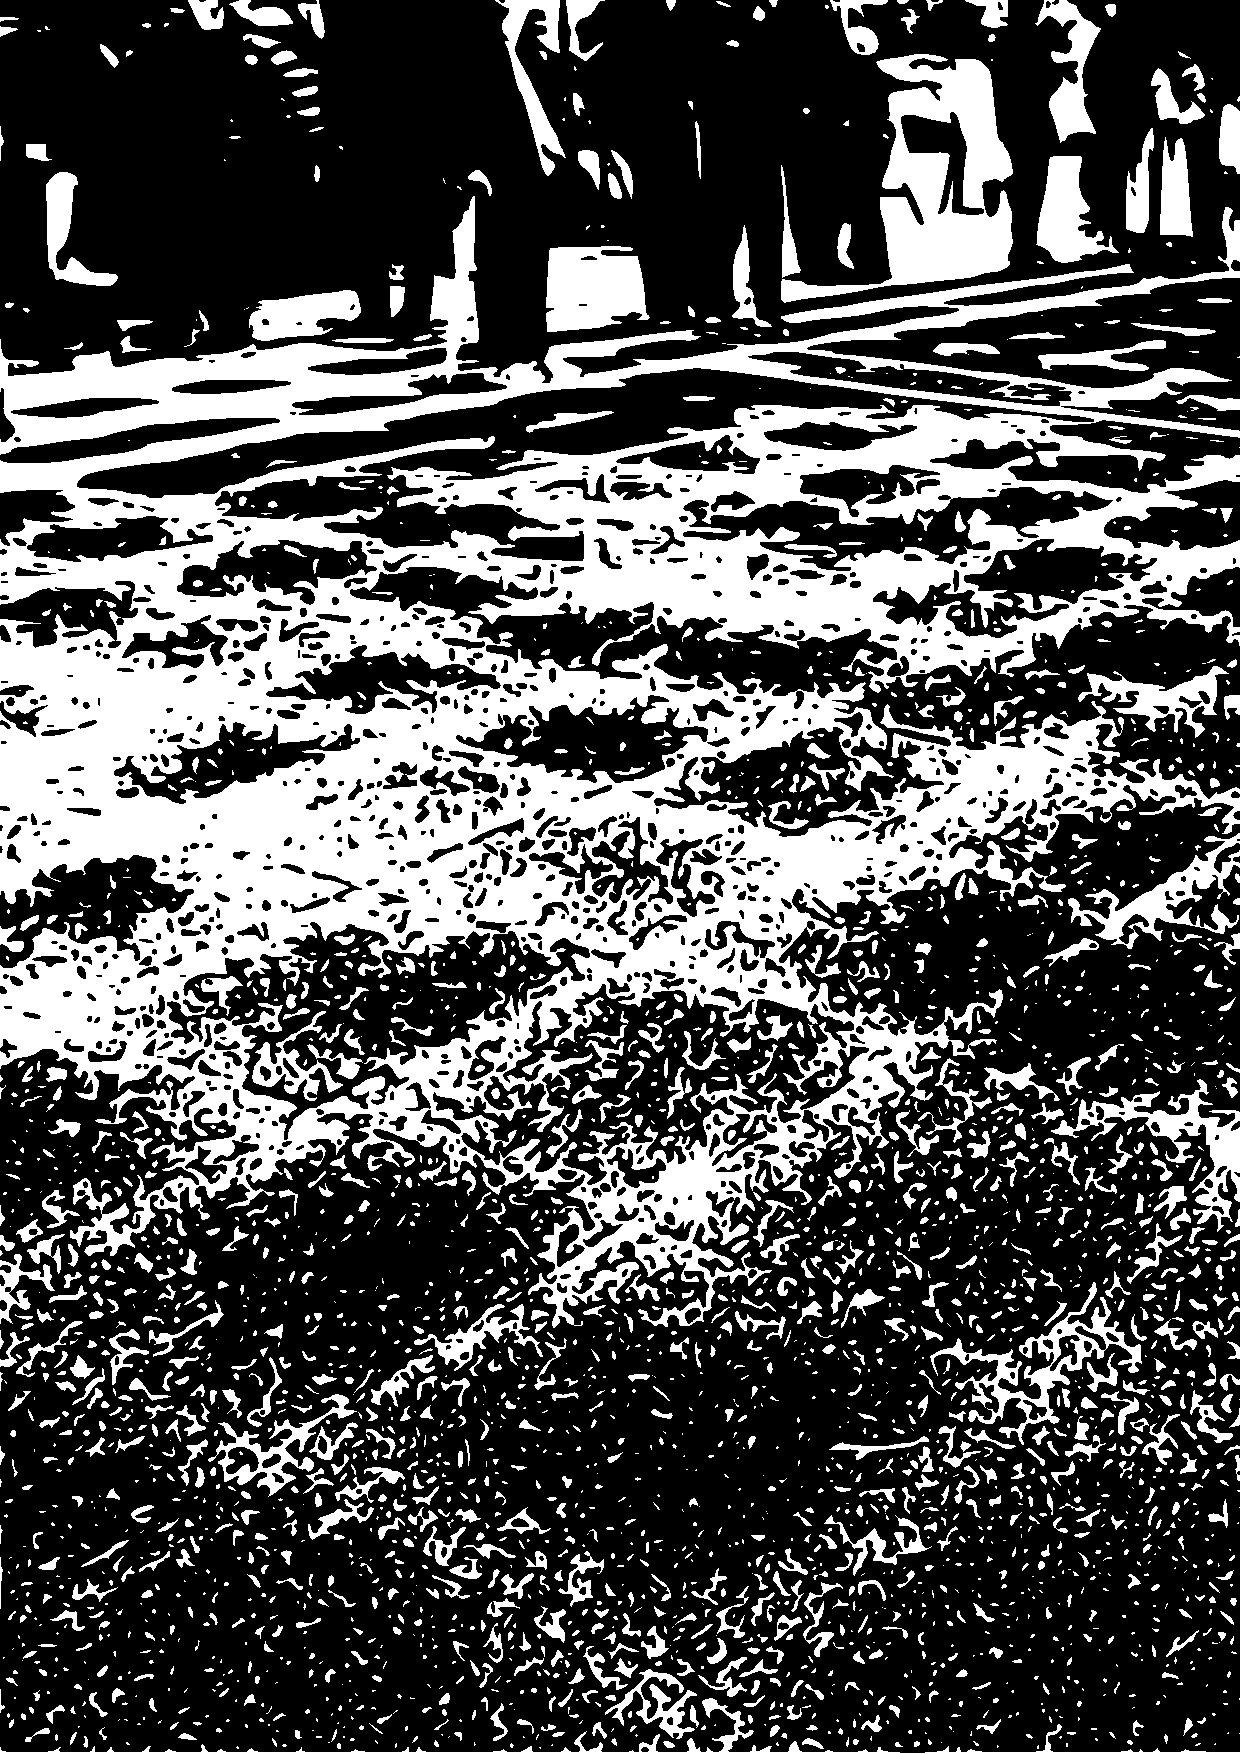
\includegraphics[width=0.8\linewidth]{fig/hitogomi.png}
   \caption{Crowds at the starting point of Tsukuba Challenge 2022}
   \label{fig:つくばチャレンジ人混み}
 \end{figure}

\section{観測範囲を制限したMCL}%===========================

実装する手法は、ひとつのパーティクルが
ベイズの定理を適用される際に使われる
LiDARの観測範囲を制限し、
パーティクルごとに、
その範囲を変えるというものである。
たとえば2次元LiDARで、ロボット前方を$0$[deg]としたときに
左右$\varphi_\text{max}$[deg]の範囲が計測できるとする。
このとき、MCLで各パーティクルの重みを変えるとき、
$\varphi^{(i)} \pm \varphi'$[deg]
の範囲の距離計測値しか用いない。
ここで$i$は$i$番目のパーティクルという意味である。
つまり、パーティクルによって使う距離計測値の範囲を変える。
また、$ -\varphi_\text{max} \le \varphi^{(i)}-\varphi'$、
$\varphi^{(i)}+\varphi' \le \varphi_\text{max}$とする。

このように観測範囲を限定し、
パーティクルごとに可変とする狙いは、
未知障害物に観測範囲が向いている
パーティクルを減らすことである。
たとえば自己位置推定が安定している状態で
ロボットが直線状の通路を前進していると、
右の路肩に地図には記載のない乗用車が
停車してあったときの状況を考える。
このとき、パーティクルのうち、
観測範囲が乗用車に向いているものは、
地図とLiDARからの値の整合性がとれず、
リサンプリングの際に消去されやすい。
この際、生き残ったパーティクルは、
複製される。
このような淘汰が進むと、
パーティクルが未知障害物の観測を避けるようになる。

この方法は、未知障害物
への対策になっていると同時に、
各パーティクルにベイズの定理を適用する
際の計算が$\Delta\varphi^{(i)}/\varphi_\text{max}$倍に減少する。
一方、LiDARからMCLへ取り込む情報が減少することや、
パーティクルの観測する向きが一方向に揃って
ロバスト性がなくなる問題の発生が懸念される。
後者については、リサンプリングの際、
$\beta$[\%]のパーティクルの観測範囲を
ランダムに変更することで対処する。
次章の実験では、$\beta=10$[\%]としている。
前者については、次章で検証する。

\section{実験}%===========================

\subsection{実験環境}

実験は、つくばチャレンジの環境を再現した
シミュレータ環境で行う。
図\ref{fig:人混みガゼボ}は、
シミュレータ内で
図\ref{fig:つくばチャレンジ人混み}
の場所、状況を再現した部分である。
図中にある壁のようなものは
ロボットが持つ地図中に記載のある障害物(既知障害物)で、
実機に搭載した2次元LiDARで得たデータをもとに配置している。
同じく図中に見られるマネキンと箱は、
図\ref{fig:つくばチャレンジ人混み}を参考に、
未知障害物として配置した。
これらの未知障害物は、静止している。

%今回使用したPCの環境を表\ref{table:PCの環境}に示す。
%シミュレータのソフトウェアとしてGazebo、ナビゲーションのシステムとしてROS Noeticを使用する。
環境については、
図\ref{fig:つくばチャレンジ人混みシミュレータ}左のように
未知障害物を置かないものと、右のように置くものの2通りを準備した。
未知障害物の数や配置は、後述のように通常のMCLでは
自己位置推定が困難になるように設定した。


それぞれの環境で、
あらかじめ筆者らがシミュレータ中の
ロボットを操作して作成した走行経路を、
ロボットが誤差なしで移動する。
この移動の際にロボットはMCLを実行する。
パーティクル数は$10,000$とする。
シミュレーション中の各時刻で、
パーティクルの位置と向きの平均値と
ロボットの位置と向きを記録する。

シミュレータ内で走行させるロボットは、
図\ref{fig:raspicat}のような差動二輪型のロボットである。
地面から高さ$0.7$[m]の位置に、観測範囲を$360$[deg]、
角度分解能を$1$[deg]の2次元LiDARを搭載している。
シミュレータ内の既知、未知障害物との距離は、
この高さで検知できるように設定されている。

%ロボットの最高速度は、3[m/s]とする。

%\begin{table}[hbtp]
%  \caption{experimental environment}
%  \label{table:PCの環境}
%  \centering
%  \begin{tabular}{ll}
%    \hline
%    \small{CPU}     & \small{Core™ i9-12900K × 24} \\
%    \small{GPU}     & \small{GeForce RTX 2060} \\
%    \small{Ubuntu}  & \small{20.04} \\
%    \small{ROS}     & \small{Noetic} \\
%    \small{Gazebo}  & \small{9.0} \\
%    \hline
%  \end{tabular}
%\end{table}

%\begin{table}[hbtp]
%  \caption{performance of the robot and on-board sensors}
%  \label{table:ロボットおよび搭載しているセンサの性能}
%  \centering
%  \begin{tabular}{lr}
%    \hline
%    \small{ロボットの最高速度}      & \small{3[m/s]} \\
%    \small{2D LiDARの取り付け高さ}  & \small{1[m]} \\
%    \small{2D LiDARの観測範囲}      & \small{360[deg]} \\
%    \small{2D LiDARの角度分解能}    & \small{1[deg]} \\
%    \hline
%  \end{tabular}
%\end{table}

\begin{figure}[htbp]
  \centering
   \includegraphics[width=0.8\linewidth]{fig/hitogomi_gazebo.png}
	\caption{A scene in the simulator imitating Fig.~\ref{fig:つくばチャレンジ人混み}} 
   \label{fig:人混みガゼボ}
\end{figure}

\begin{figure}[htbp]
  \centering
   \includegraphics[width=1.0\linewidth]{fig/environment_comparison.png}
	\caption{Environments without (left) and with (right) unknown obstacles}
   \label{fig:つくばチャレンジ人混みシミュレータ}
\end{figure}

\begin{figure}[htbp]
  \centering
   \includegraphics[width=0.5\linewidth]{fig/raspicat_gazebo.png}
   \caption{The robot running in the simulator}
   \label{fig:raspicat}
\end{figure}

\subsection{誤差の評価}


様々な観測範囲$\varphi'$でロボットを走行させて、
自己位置推定の正確さを比較した。
図\ref{fig:つくばチャレンジ人混みシミュレータ}左の
未知障害物を置かない場合と、右のように置く場合を100回ずつ、
各観測範囲で試行して誤差を記録した
結果を表\ref{table:error}に示す。
これらの値は、距離、向きの誤差のうち、
距離の誤差を100回の試行中の各時刻で平均したものである。
ここで言う距離の誤差とは、
パーティクルの位置の平均値と、
ロボットの位置の距離のことを指す。

\begin{table}[htbp]
	\centering
	\caption{Comparison of average errors without/with obstacles}
  \label{table:error}
	\begin{small}
  \begin{tabular}{|r|r|r|r|} \hline
	  field of view & \multicolumn{2}{c|}{error[m]} \\
	  $2\varphi'$[deg]  & without obstacles & with obstacles \\ \hline \hline
	  {0}         & \textit{2.29} & 2.11 \\ \hline
	  {1}         & 0.54 &  \textbf{1.94} \\ \hline
	  {10}        & 0.50 & \textbf{0.88} \\ \hline
	  {45}        & 0.38 & 5.89 \\ \hline
	  {90}        & \textbf{0.37} & \textit{8.44}\\ \hline
	  {360}       & \textbf{0.32} & 5.65 \\ \hline
  \end{tabular}
	\end{small}
\end{table}


表のように、未知障害物がない場合は
観測範囲を狭くすると誤差が大きくなる傾向が
見られたが、未知障害物が多いと
観測範囲が$2\varphi'=1$[deg]、$10$[deg]
など、極端に狭めた場合のほうが誤差が小さいという結果となった。
つまり、提案手法が有効に機能したと考られる。


図\ref{fig:スタートからゴールまでナビゲーション}は、
$2\varphi'=1$[deg]のとき、
LiDARのレーザーがどの障害物に当たっていたかを集計したものである。
緑色が$2\varphi'=1$[deg]の範囲に入って自己位置推定に使用された
レーザーの当たった箇所、赤色が範囲外のレーザーの当たった箇所である。
緑色の部分は地図に記載のある障害物を捉えており、
一方、赤色は未知障害物の表面に分布している。
これを見ると、提案手法で未知障害物の観測を避ける仕組みが
機能していると考えられる。

また、観測範囲がこれより大きくなると、
緑色の範囲はより広くぼやけて、
未知障害物の表面まで分布するようになると考えられる。
そのため、表\ref{table:error}のように、
$2\varphi'=45$[deg]や$2\varphi'=90$[deg]のときは、
十分に提案手法の効果が得られなかったものと考えられる。



%自己位置推定の破綻とは、
%MCLのパーティクルが実際のロボットの位置からなくなり、
%ロボットがどこを走っているのか間違え、さらに修正不能に
%陥る状況のことを指す。
%本稿の実験では、目視でこの状態に陥ったかどうかを判断した。
%具体的には、パーティクルの位置、向きの平均値を
%基準にLiDARの計測値を地図に重ね、
%図\ref{fig:スタートからゴールまでナビゲーション}右の
%丸で囲った部分から計測値が外れて元にもどらなくなったときを
%破綻と判断した。
%なお、シミュレーションではロボットが
%移動の際に雑音を受けないことから、
%自己位置推定の破綻と判断されても、
%
%
%このナビゲーション自体は簡単なものであるが、
%MCLが破綻すると、完走できない。

%未知障害物の配置や数については、
%後述の結果のように、通常のMCLでは
%推定が破綻するように調整した。


%観測範囲を変えて、それぞれの観測範囲で
%$100$回試行した結果を表\ref{table:完走率}
%に示す。センサを用いない場合($2\varphi' = 0$[deg])
%や観測範囲に制限を設けない場合($2\varphi' = 360$[deg])
%は、完走した試行が一度もなかった。
%一方、$2\varphi' = 1$[deg]と極端に観測範囲を狭めた場合の
%完走率は$28$[\%]、
%$2\varphi' = 10$[deg]の場合については$54$[\%]となった。

\begin{figure}[t]
  \centering
   \includegraphics[width=0.8\linewidth]{fig/particle_1000_observation_1_mcl.png}
   \caption{Navigation from start to finish (left) and visualization of observations used in the observation update (right)}
   \label{fig:スタートからゴールまでナビゲーション}
\end{figure}

%\begin{table}[htbp]
%	\centering
%	\caption{Relation between the observation range and the number of success trials}
%  \label{table:破綻率}
%	\begin{small}
%  \begin{tabular}{|r|r|r|r|} \hline
%	  $2\varphi'$[deg]  & \small{破綻率}[\%] \\ \hline \hline
%  {0}         & 100 \\ \hline
%  {1}         & 72 \\ \hline
%  {10}        & 46 \\ \hline
%  {45}        & 96 \\ \hline
%  {90}        & 100 \\ \hline
%  {360}       & 100 \\ \hline
%  \end{tabular}
%	\end{small}
%\end{table}
%
%図\ref{fig:スタートからゴールまでナビゲーション}右は、
%観測範囲が$2\varphi' = 1$[deg]のときに、
%観測対象となった距離計測値と、
%ならなかった距離計測値を、
%障害物上にプロットしたものである。
%観測対象となった距離計測値は、MCLの周期たびに、
%全てのパーティクルで使用されている観測範囲の最頻値として求めたものである。
%緑色が観測対象となった距離計測値で、
%ほとんどが既知障害物を計測したものとなっている。
%2章の手法で、未知障害物を計測した値を
%除去することが可能であることが分かる。
%
%
%
%
%実験方法は以下のとおりである。
%\noindent
%\begin{enumerate}[A]
%  \item スタートからゴールまでオンラインでロボットのナビゲーションをする
%  \item 事前にジョイスティックでロボットをスタートからゴールまで動かす。
%        その間、得られた観測情報等を記録したデータを後から再生し、オフラインで自己位置推定をする。
%\end{enumerate}
%\noindent
%スタートとゴールは、それぞれ図\ref{fig:スタートからゴールまでナビゲーション}
%に示された位置である。

%今回の実験の評価項目は、以下のとおりである。
%\begin{itemize}
%  \item スタートからゴールまでの100回ナビゲーションさせた場合の完走率(実験方法A)
%  \item スタートからゴールまで走行したときの真値との比較(実験方法B)
%  \item パーティクルの観測更新に最も使用された観測(実験方法A)
%  % \item 計算時間の増減(実験方法A)
%\end{itemize}


%表\ref{table:完走率}に、実験方法Aにより求めた、各パーティクルの条件での完走率を示す。
%結果からは、観測範囲が狭くなるほど完走率が大きくなっていることがわかる。

%\begin{table}[htbp]
%  \caption{completion rate under certain particle conditions}
%  \label{table:完走率2}
%  \begin{tabular}{|r|r|r|r|} \hline
%  \small{条件番号} & \small{パーティクル数} & \small{観測範囲}  & \small{完走確率} \\ \hline \hline
%  \small{\textcircled{\scriptsize 1}}  & \small{3000}  & \small{0[deg]}         & \small{0.00} \\ \hline
%  \small{\textcircled{\scriptsize 2}}  & \small{3000}  & \small{10[deg]}        & \small{0.52} \\ \hline
%  \small{\textcircled{\scriptsize 3}}  & \small{3000}  & \small{360[deg]}       & \small{0.00} \\ \hline
%  \small{\textcircled{\scriptsize 4}}  & \small{10000} & \small{0[deg]}         & \small{0.00} \\ \hline
%  \small{\textcircled{\scriptsize 5}}  & \small{10000} & \small{1[deg]}         & \small{0.28} \\ \hline
%  \small{\textcircled{\scriptsize 6}}  & \small{10000} & \small{10[deg]}        & \small{0.54} \\ \hline
%  \small{\textcircled{\scriptsize 7}}  & \small{10000} & \small{45[deg]}        & \small{0.04} \\ \hline
%  \small{\textcircled{\scriptsize 8}}  & \small{10000} & \small{90[deg]}        & \small{0.00} \\ \hline
%  \small{\textcircled{\scriptsize 9}}  & \small{10000} & \small{360[deg]}       & \small{0.00} \\ \hline
%  \small{\textcircled{\scriptsize 10}} & \small{10000} & \small{1$\sim$15[deg]} & \small{0.54} \\ \hline
%  \end{tabular}
%\end{table}
%
%各パーティクルの条件において、自己位置推定が破綻した場所を
%図\ref{fig:失敗箇所}に示す。
%\textcircled{\scriptsize 3}\textcircled{\scriptsize 5}\noindent
%\textcircled{\scriptsize 8}\textcircled{\scriptsize 9}\noindent
%の条件は、スタートから12[m]あたり、
%\textcircled{\scriptsize 2}\textcircled{\scriptsize 6}\noindent
%\textcircled{\scriptsize 7}\textcircled{\scriptsize 10}\noindent
%の条件は、スタートから30[m]のあたりで
%自己位置推定が破綻することがあった。

%\begin{figure}[htbp]
%  \centering
%   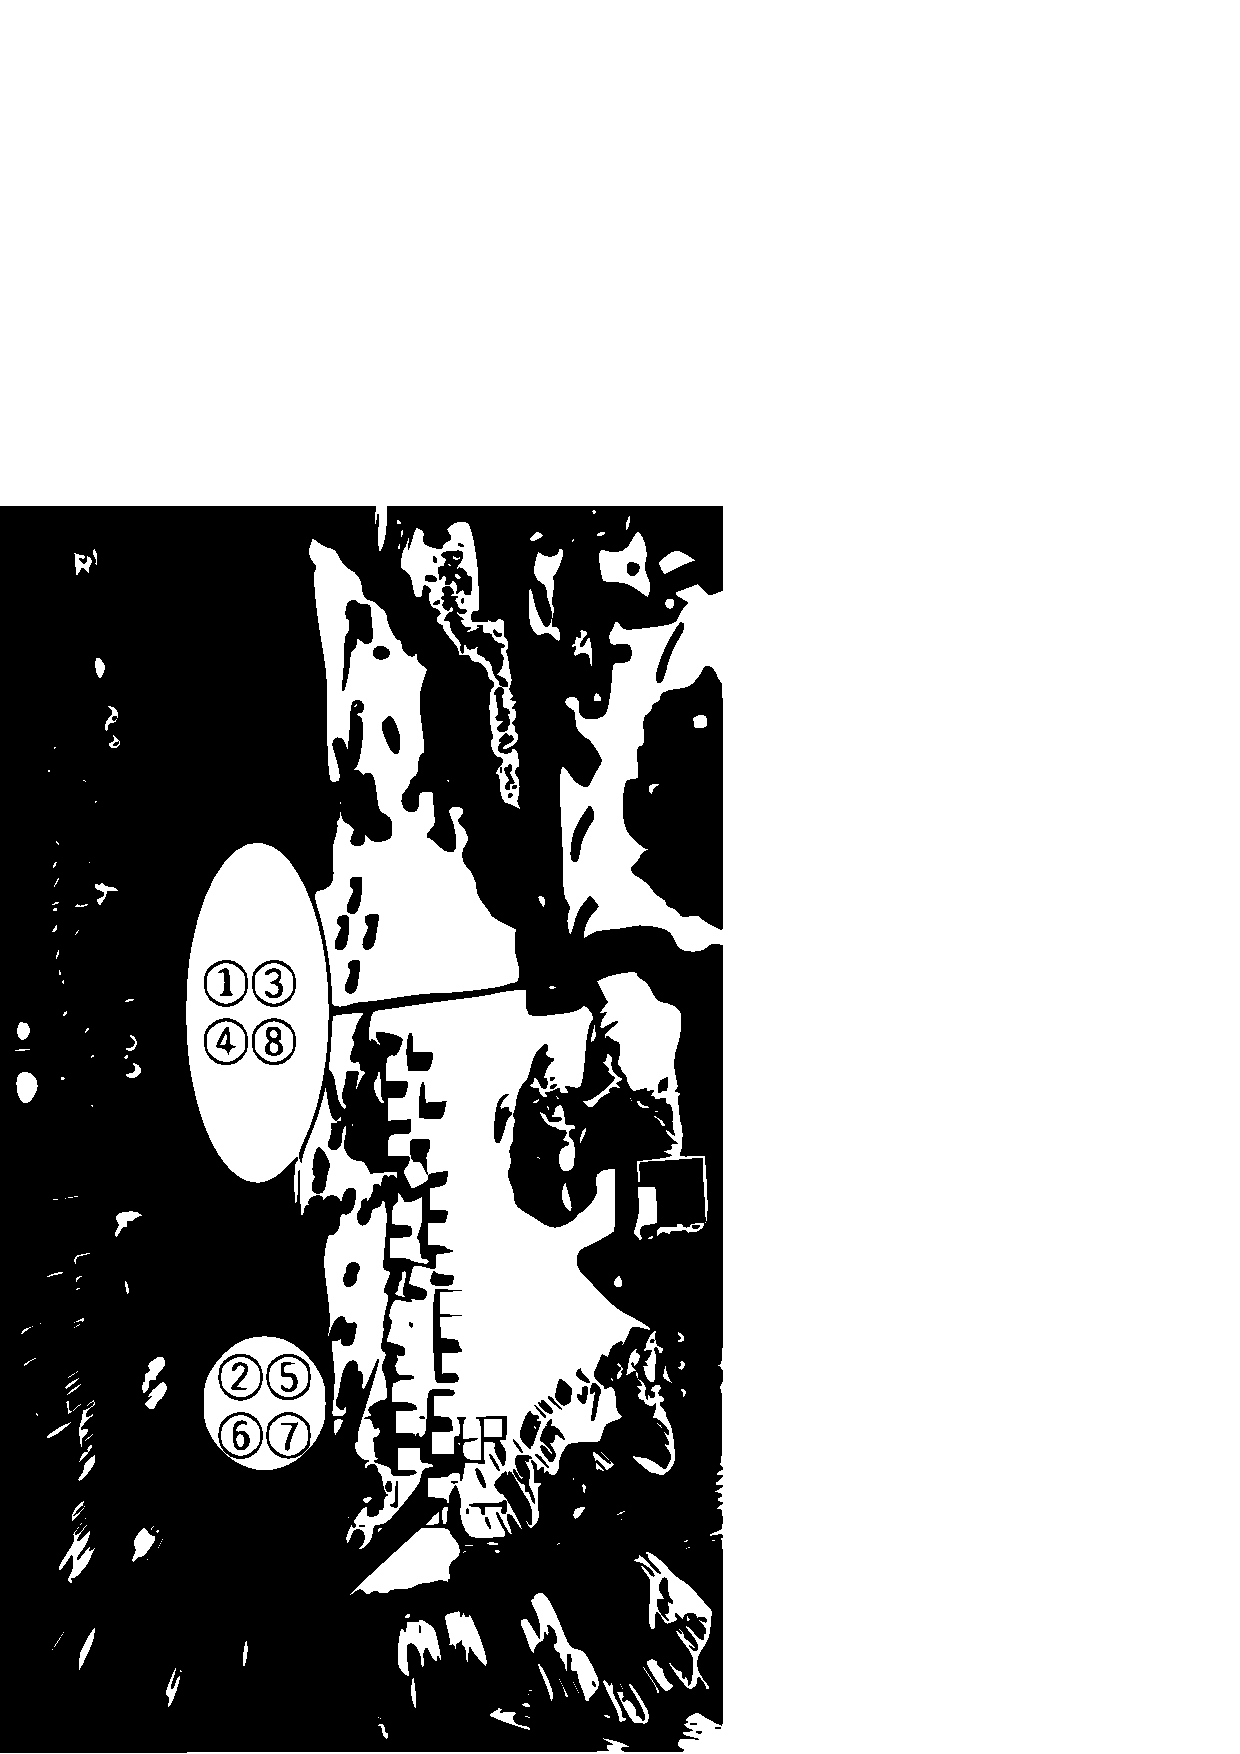
\includegraphics[width=0.8\linewidth]{fig/failure_location.png}
%   \vspace*{-4mm}
%   \caption{Where localization has broken down}
%   \label{fig:失敗箇所}
%\end{figure}

%\subsection{自己位置推定の誤差}
%
%図\ref{fig:plot}に、実験方法Bにより求めた、
%真値(reference)に対する各パーティクルの条件での
%自己位置推定値の誤差を示す。
%まず、xy平面上に真値と自己位置推定をプロットしたものを見ると、
%条件
%\textcircled{\scriptsize 3}\textcircled{\scriptsize 7}\noindent
%\textcircled{\scriptsize 8}\textcircled{\scriptsize 9}\noindent
%の場合、スタートから約10[m]の場所から自己位置の推定誤差が大きくなり、自己位置推定破綻を起こした。
%条件
%\textcircled{\scriptsize 1}\textcircled{\scriptsize 4}\noindent
%の場合、スタートから約19[m]の場所から自己位置の推定誤差が大きくなり、自己位置推定破綻を起こした。
%条件
%\textcircled{\scriptsize 2}\textcircled{\scriptsize 5}\noindent
%\textcircled{\scriptsize 6}\textcircled{\scriptsize 10}\noindent
%は、スタートから約15$\sim$20[m]の場所から自己位置の推定誤差が大きくなり始めたが、
%20[m]以降は一定の誤差のままゴールまで到達した。
%中でも条件
%\textcircled{\scriptsize 5}\noindent
%の誤差が小さいように見える。
%
%xy平面上に真値と自己位置推定をプロットしたものの中でも
%自己位置の推定誤差が小さかった4つの条件
%\textcircled{\scriptsize 2}\textcircled{\scriptsize 5}\noindent
%\textcircled{\scriptsize 6}\textcircled{\scriptsize 10}\noindent
%において、真値に対する自己位置推定値のユークリッド誤差、横誤差、縦誤差
%をプロットした。
%4つの条件の中でも、条件
%\textcircled{\scriptsize 2}\textcircled{\scriptsize 5}\noindent
%の誤差が小さいように見える。
%しかし、誤差が小さいといっても、それぞれの条件において、
%最大で横誤差が0.4[m]、縦誤差が0.8[m]、ユークリッド誤差が0.8[m]もある。

%\begin{figure}[htbp]
%  \begin{center}
%  \begin{tabular}{cc}
%  \includegraphics[width=0.8\linewidth]{fig/x_y.png} \\
%  \includegraphics[width=0.8\linewidth]{fig/euclidean_error.png} \\
%  \includegraphics[width=0.8\linewidth]{fig/lateral_error.png} \\
%  \includegraphics[width=0.8\linewidth]{fig/longitudinal_error.png} 
%  \end{tabular}
%  \caption{
%    Plot the true value and the self-estimated position value,
%     and the lateral direction and the longitudinal 
%    direction and Euclidean error with respect to the true value.}
%  \label{fig:plot}
%  \end{center}
%\end{figure}
%
%\subsection{使用される観測}

%2章で説明した手法をMCLに実装すると、
%各パーティクルは観測範囲を持ち、
%未知障害物が含まれないような観測を
%パーティクルの観測更新に使用するようになる。
%図\ref{fig:スタートからゴールまでナビゲーション}の左の図のようにロボットを
%スタートからゴールまでナビゲーションをさせた時
%観測更新においてどの観測を使用していたか、可視化したものを
%図\ref{fig:スタートからゴールまでナビゲーション}の右の図に示す。
%このときのパーティクルの条件は、パーティクルの数10000、観測範囲1[deg]である。
%赤色が、スタートからゴールまでの全観測であり、
%緑色が、手法の実装によって既知障害物の観測として求められた観測である。
%未知障害物の観測であるのに緑色になっている部分が少しあるが、
%ほとんど既知障害物の観測を選択していることがわかる。


% \subsection{実装による計算時間の増減}

% 自己位置の推定誤差が小さかった4つの条件
% \textcircled{\scriptsize 2}\textcircled{\scriptsize 5}\noindent
% \textcircled{\scriptsize 6}\textcircled{\scriptsize 10}\noindent
% と、元のMCLと同じ条件である
% \textcircled{\scriptsize 3}\noindent
% において、観測更新の計算時間を計測した。
% 計測した時間の結果を表\ref{table:観測更新の計算時間}に示す。
% 条件
% \textcircled{\scriptsize 3}\textcircled{\scriptsize 2}\noindent
% の結果を比較すると、観測範囲を狭めた場合、
% 実装以前よりも計算時間が減少することがわかった。
% また、パーティクルを3000から10000個に増やした時の計算時間は
% \textcircled{\scriptsize 2}\textcircled{\scriptsize 6}\noindent
% 相関して、3倍に増加していることがわかる。

% \begin{table}[htbp]
%   \caption{Computation time for observation updates under each particle condition}
%   \label{table:観測更新の計算時間}
%   \centering
%   \begin{tabular}{|c|r|r|r|} \hline
%   条件番号 & 平均[ms] & 標準偏差[ms]  \\ \hline \hline
%   \textcircled{\scriptsize 3} & 8.6 & 2.0   \\ \hline
%   \textcircled{\scriptsize 2} & 8.0 & 1.0   \\ \hline
%   \textcircled{\scriptsize 6} & 25.9 & 1.71 \\ \hline
%   \textcircled{\scriptsize 10} & 28.1 & 1.9  \\ \hline
%   \end{tabular}
% \end{table}


\section{結言}%===========================

本稿では、MCLとLiDARを組み合わせて自己位置推定するときに、
未知障害物を計測したセンサ値を省く仕組みを提案し、
評価した。具体的な方法は、
各パーティクルごとに2次元LiDARの観測範囲を制限し、
観測する方向をランダムに変えるというものである。
シミュレータ内に構築した未知障害物の多い環境で、
数種類の観測範囲を試したところ、
$360$[deg]観測可能なLiDARに対し、$1$[deg]や$10$[deg]など、
極端に観測範囲を制限したほうが良好な結果が得られた。


今後は、観測範囲を制限することで起こる
悪影響はないかを確認するために、
実環境やシミュレータ環境で、様々な
未知障害物の存在下の状況で実験を重ねる。
また、観測範囲を制限したことで
計算量が減少しているはずであるが未検証なので、
この点についても調査する。

%付与した場合のMCLの性能や良さそうな条件を実験により求めた。

%本稿では、各パーティクルごとにランダムな観測範囲を
%付与した場合のMCLの性能や良さそうな条件を実験により求めた。
%実験結果からは、各パーティクルごとにランダムな観測範囲を
%付与した場合のMCLは、パーティクルに付与する観測範囲が狭いほど、
%未知障害物が多く存在する環境下での、自己位置の推定性能が高いことがわかった。
%また、完走率が低くなってしまっているが、パーティクルに付与する観測範囲が狭い条件で、
%パーティクルの数を増やすことで自己位置の推定誤差を小さくできる可能性があることがわかった。


\footnotesize
\begin{thebibliography}{99}

  \bibitem{gutmann2002}
  Jens-Steffen Gutmann and Dieter Fox, 
  ``An Experimental Comparison of Localization Methods Continued,''
  Proc. IEEE/RSJ International Conference on Intelligent Robots and Systems (IROS), pp.~454-459, 2002.

  \bibitem{つくばチャレンジ}
  油田信一, ``つくばチャレンジ: 市街地における移動ロボットの自律走行の公開実験 ---11 年の経緯と成果---'',
  第23回ロボティクスシンポジア講演論文集, (2018), pp.~59-66.
  
  \bibitem{富沢2012}
  冨沢哲雄, 村松聡, 平井雅尊, 佐藤晶則, 工藤俊亮, 末廣尚士, 
  ``グリッドマップのマッチングに基づく未知障害物にロバストな自己位置推定'', 日本ロボット学会誌, Vol.~30, No.~3, pp.~280-286, 2012.
  
  \bibitem{赤井2019}
  赤井直紀, モラレスルイス洋一, 平山高嗣, 村瀬洋, 
  ``幾何地図上での観測物体の有無を考慮した自己位置推定'', 計測自動制御学会論文集, Vol.~55, No.~11, pp.~745-753, 2019.
  
%  \bibitem{ROS}
%Morgan Quigley {\it et al.}: ``ROS: an open-source Robot Operating System,'' 
%Open-Source Software workshop of the International Conference on Robotics and Automation (ICRA), 2009. 

\end{thebibliography}

\normalsize
\end{document}
